\section{Categorization of PUTs}
\label{sec:categorization}

We used suggested test patterns~\cite{halleux08:putpatterns} 
to generalize conventional unit tests. These test patterns can help developers in writing effective PUTs. Although PUTs alleviate the problem of writing different conventional unit tests to test the code under test with different input values, writing test oracles in PUTs could be a complex task. The developers are expected to specify sufficient assertions for testing various expected behaviors of executing the code under test. To deal with this complexity, developers can use test patterns to answer important questions of ``what'' scenarios of the code under test need to be tested and ``how'' they can be asserted. In our study, we found that a few test patterns are predominantly applicable while others are helpful in a few specific cases. 
In addition, we found that each PUT can be categorized into more than
one test pattern. In all, the patterns supported by Pex help write a wide range of PUTs for achieving high code coverage and reduce
PUT writing effort for both test-driven development and testing after the application is developed. 
We found that it was not easy to write PUTs for a few scenarios of the code under test using these patterns. To address this issue, we proposed two new patterns that can help in writing PUTs. We first explain the categories of the existing patterns as \textit{used} and \textit{not used} based on whether there are PUTs that belong to the test pattern and later present our proposed new patterns.
%---------------------------------------------------------------------------------------
\subsection{Existing Test Patterns}

We next present the classification of our PUTs into existing test patterns. Table~\ref{tab:patterns} shows the $15$ existing test patterns~\cite{halleux08:putpatterns}. Column 1 provides the classification of each pattern in our study. We put the existing test patterns into two categories based on their usage in this study: used and not used. Column 2 provides the pattern identifier. We use these identifiers to refer to the patterns in this section. Column 3 provides the pattern name and Column 4 gives the attributes\footnote{Pex provides a set of custom attributes to tag test class, test methods or parameters.} and methods supported by Pex for that pattern. 

\setlength{\tabcolsep}{2pt}
\begin{table*}[t]
\begin{center}
\centering \caption {\label{tab:patterns} Existing Test Patterns Supported By Pex.} \vspace*{0.1in}
\begin {tabular} {|l|r|l|l|}
\hline
Category					&	Pattern\#	&	Pattern Name												&	Pex Supported Attributes or Methods\\
\hline
Used							&	2.1				&	Arrange, Act, Assert								&	\\
\cline{2-4}
									& 2.2				&	Assume, Arrange, Act, Assert  			&	\\
\cline{2-4}
									&	2.3				&	Constructor Test										&	\\
\cline{2-4}
									& 2.4				&	Roundtrip														&	\\
\cline{2-4}
									& 2.5				&	Sanitized Roundtrip									&	\\
\cline{2-4}
									& 2.6				&	State Relation											&	\\
\cline{2-4}
									&	2.7				&	Same Observable Behavior						&	\\
\cline{2-4}
									&	2.8				&	Commutative Diagram									&	\\
\cline{2-4}
									& 2.9				&	Cases																&	PexAssert.Case() 			\\ 
\hline
Not used					& 2.10			&	Allowed Exception										&	[PexAllowedException]	\\
\cline{2-4}
									& 2.11			&	PexAllowedException									&	[PexExpectedGoals]		\\
\cline{2-4}
									&	2.12			&	Parameterized Stub									&	[PexAssumeUnderTest]	\\
\cline{2-4}
									&	2.13			&	Manual Output Review								&	PexStore.Value()			\\
\cline{2-4}
									&	2.14			&	Regression Tests										&	PexStore.ValueForValidation()\\
\cline{2-4}			
									& 2.15			&	Differential Regression Test Suite	&	\\
\hline
\end{tabular}
\end{center}
\end{table*}

\begin{enumerate}
\item \textbf{Used}: We put a pattern under this category if that
pattern was used at least once when writing PUTs.
We used 9 Patterns (from Pattern 2.1 to 2.9) for writing PUTs. Figure~\ref{fig:patterndistribution} shows the 
distribution of pattern usage across all the 70 PUTs. The x axis of the 
chart shows the used patterns and the y axis shows the number of PUTs that belong to each pattern.
For each test pattern, we show the number of PUTs in our study. 

\item \textbf{Not used}: We put a pattern under this category if that 
pattern was not used in test generalization. We found that $5$ 
out of the $15$ patterns were not used in writing PUTs in our study  
(from 2.10 to 2.15). The possible reason for not using these patterns 
in our test generalization is the lack of purposes for these patterns 
in our current study. For example, Patterns 2.14 and 2.15 are applied 
in the context of regression testing. However, in our current study, our
focus is not on regression testing. 
\end{enumerate}

\begin{figure}[t]
\centering
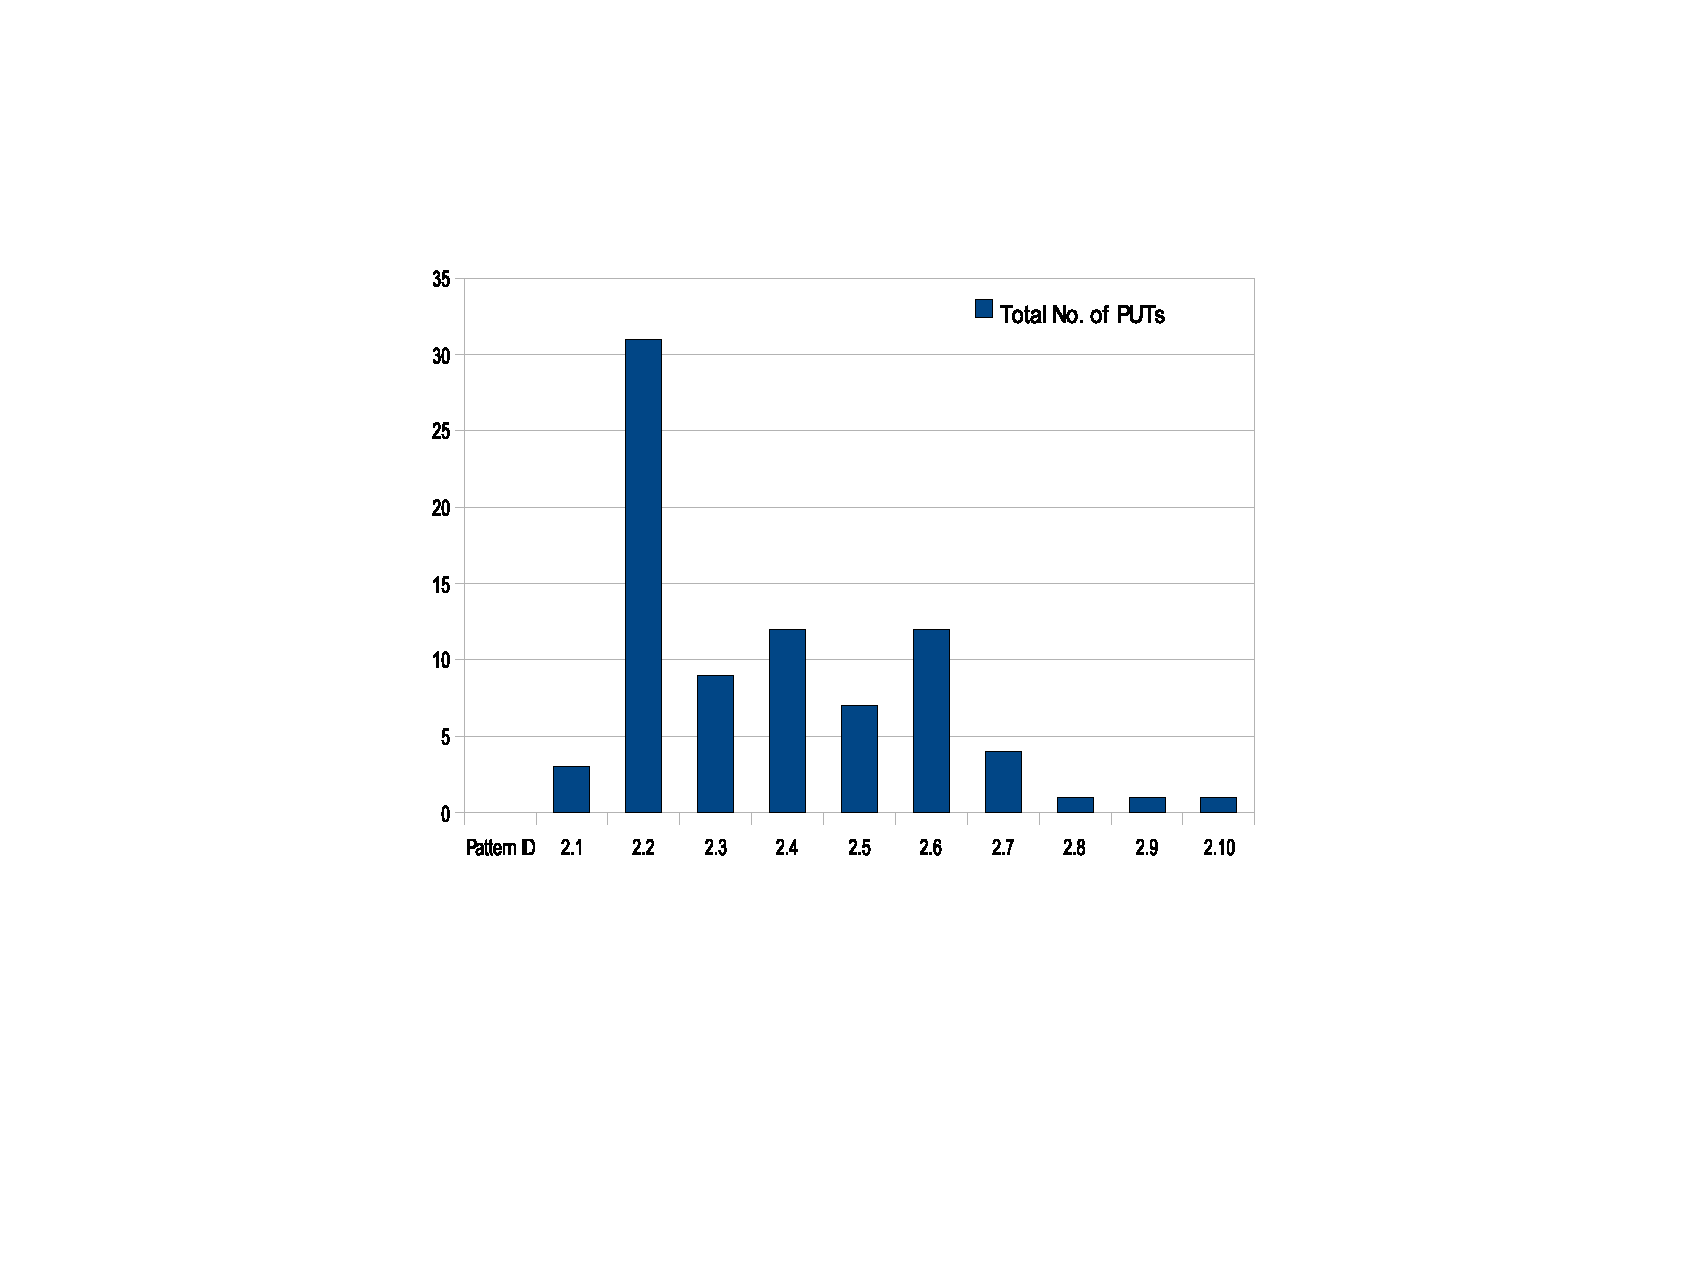
\includegraphics[scale=0.55,clip,trim=180 180 150 100]{figs/patterndistributionSeparated.eps}
\caption{\label{fig:patterndistribution}Distribution of test patterns for 70 PUTs. \textit{The distribution shows that in our testing, only patterns from 2.1 to 2.9 were used.}}
\end{figure}
%---------------------------------------------------------------------------------------
\subsection{New Patterns}
\label{sec:newpatterns}

We next describe two new patterns that can be supported, and that we found useful during our test generalization for the NUnit framework. 
%-------------------------------------------------------------------------------------------
\subsubsection{Random Selection of Cached Values}
\emph{Purpose}: To reuse generated values by maintaining a pool and randomly picking from those values.
\newline
\emph{Motivation}: We next show the motivation for such a pattern with an illustrative example. In the test generalization phase, we needed to generalize an existing unit test 
that requires to verify whether adding a \CodeIn{RegisterKey} to an \CodeIn{NUnitRegistry} and 
then clearing the \CodeIn{NUnitRegistry} work as expected. The \CodeIn{NUnitRegistry} class holds \CodeIn{RegisterKeys} as a tree structure with a main key and an unrestricted number of subkeys in a tree-structured form. Manually adding values and creating a tree structure to check both horizontal and vertical cases at the same time was possible in the existing conventional unit test. However, when the test was parameterized, we were able to write a PUT to add all \CodeIn{RegisterKeys} either to one main key or add each \CodeIn{RegisterKey} to the last added key. Due to such restriction, the unit tests generated by this PUT
resulted in a reduced block coverage when compared to the conventional unit test, although there are a number of tests generated for the PUT. The rationale is that the tests generated for the PUT are expected to generate
a tree structure of keys to achieve high code coverage. As the existing test 
patterns do not meet our current requirement, we proposed a new pattern
where we maintain a pool of existing \CodeIn{RegisterKeys} and randomly
select a key from this pool to add the newly created key as a subkey.
Our new pattern can help construct several forms of tree structures automatically.
Although we explain our motivation using the \CodeIn{RegisterKeys} test
example, our pattern is general and can be applied to tests that require
to reuse previously generated values.
\newline
\emph{Proposed Pattern}: When the input is of the type collection or an array and the values need to be reused by the code under test, 
the values generated by Pex can be added to a pool using our proposed method 
\CodeIn{PexStore.Pool(<name>,<value>)}. \CodeIn{PexStore.Pool()} method is expected to cache values (represented by \CodeIn{value}) for a particular variable (represented by \CodeIn{<name>}). Later, a value can be picked randomly from these cached values using another proposed method \CodeIn{PexStore.Pick(<name>)}. \CodeIn{PexStore.Pick()} method is expected to pick a value randomly from the cached store of the variable \CodeIn{<name>}. Figure~\ref{fig:treepattern} shows an application of our proposed pattern.

\begin{figure}[t]
\begin{CodeOut}
\begin{alltt}
00:[PexMethod()]
01:public void TestClearRoutinesPUT([PAUT]String[] key) \{
02:\hspace*{0.1in}PexAssume.IsTrue(key.Length > 1);
03:\hspace*{0.1in}for (int j = 0; j < key.Length; j++) \{
04:\hspace*{0.3in}PexAssume.IsNotNull(key[j]);
05:\hspace*{0.1in}\}
06:\hspace*{0.1in}NUnitRegistry.TestMode = true;
07:\hspace*{0.1in}using (RegistryKey mainKey = 
08:\hspace*{0.3in}NUnitRegistry.CurrentUser) \{
09:\hspace*{0.3in}//enabling appending values to a list
10:\hspace*{0.3in}\textbf{PexStore.Pool("keys",mainKey)}; 
11:\hspace*{0.3in}for (int j = 0; j < key.Length; j++) \{
12:\hspace*{0.5in}RegisterKey parentKey = 
13:\hspace*{0.7in}\textbf{PexStore.Pick("keys")} as RegisterKey;
14:\hspace*{0.5in}RegistryKey subKey = 
15:\hspace*{0.7in}mainKey.CreateSubKey(key[k - 1]);
16:\hspace*{0.5in}\textbf{PexStore.Pool("keys",subKey)};
17:\hspace*{0.3in}\}
18:\hspace*{0.3in}NUnitRegistry.ClearTestKeys();
19:\hspace*{0.3in}PexAssert.IsTrue(mainKey.SubKeyCount == 0);
20:\hspace*{0.1in}\}
21:\}
\end{alltt}
\end{CodeOut}
\Caption{A new test pattern that helps reuse previously generated values using a cache. \textit{The \CodeIn{PexStore.Pool()} method can be used to append the value \CodeIn{mainKey} to the cache of variable~\CodeIn{keys} and \CodeIn{PexStore.Pick()} method can be used to pick a random value from the cache of the variable \CodeIn{keys}}.}\label{fig:treepattern}
\end{figure}
%------------------------------------------------------------------------------------------------------------
\subsubsection{Unique-value generation}
\emph{Purpose}: To generate unique values when a parameter is a collection of values instead of a single value.
\newline
\emph{Motivation}: In our test generalization phase, for four PUTs, we were unable to achieve the same test effectiveness (i.e., block coverage) by the generated conventional unit tests as that of the existing unit tests. We found the reason to be a required object state: the required object state for the four PUTs to achieve high block coverage can be created only when a unique set of elements is available. For such PUTs, we had to write additional
code to ensure that Pex generates only unique values. For example, in the following PUT, we include a \CodeIn{for} loop with a \CodeIn{PexAssume} (as shown below) on each element of the collection to make sure that
Pex generates a set of unique values. 

\begin{CodeOut}
\begin{alltt}
//PAUT: PexAssumeUnderTest
01:public void SubstorageSettingsPUT1(
\hspace*{0.3in}[PAUT]String subName, [PAUT]String[] name)
02:\{
03:\hspace*{0.3in}PexAssume.IsNotNull(value); 
04:\hspace*{0.3in}PexAssume.IsTrue(name.Length == value.Length);
\hspace*{0.4in}/*assist Pex to generate unique values by 
							 **iterating over each array element and adding
							 **the assumption it is not equal to any other 
							 **array element*/
05:\hspace*{0.3in}for (int i = 0; i < name.Length; i++) \{
06:\hspace*{0.5in}for (int j = 0; j < name.Length; j++) \{
07:\hspace*{0.6in}PexAssume.IsFalse(name[i].Equals(name[j]));
08:\hspace*{0.5in}\}
09:\hspace*{0.3in}\}
10:\hspace*{0.1in}......
11:\}
\end{alltt}
\end{CodeOut}

\emph{Proposed Pattern}: When the input is of the type collection or an array, 
we propose a new pattern using a custom attribute called \CodeIn{PexGenerateUnique} that can inform
Pex to generate unique values. For example, applying the proposed pattern to the preceding example can
result in the following easy-to-write code. We also assume that 
\CodeIn{PexGenerateUnique} subsumes the properties of \CodeIn{PexAssumeUnderTest}.

\begin{CodeOut}
\begin{alltt}
//PAUT: PexAssumeUnderTest
01: public void SubstorageSettingsPUT1([PAUT]String 
\hspace*{0.3in}subName, [\textbf{PexGenerateUnique}]String[] name)
02:\{
03:\hspace*{0.3in}PexAssume.IsNotNull(value); 
04:\hspace*{0.3in}PexAssume.IsTrue(name.Length == value.Length);
05:\hspace*{0.1in}.....
06:\}
\end{alltt}
\end{CodeOut}

For the four PUTs that required generation of a set of unique values, we could apply the proposed pattern as shown in the preceding code example and achieve the test effectiveness.
